\documentclass{article}

\makeatletter
\renewcommand{\fnum@figure}{Εικόνα \thefigure}
\makeatother

\usepackage[greek, english]{babel}
\usepackage{alphabeta}
\usepackage{atbegshi, picture}

% Set page size and margins
% Replace `letterpaper' with`a4paper' for UK/EU standard size
\usepackage[letterpaper,top=2cm,bottom=2cm,left=3cm,right=3cm,marginparwidth=1.75cm]{geometry}

% Useful packages
\usepackage{amsmath}
\usepackage{graphicx}
\usepackage[colorlinks=true, allcolors=blue]{hyperref}
\usepackage[utf8]{inputenc}
\usepackage{indentfirst}

\newcommand\T{\rule{0pt}{2.6ex}}       % Top strut
\newcommand\B{\rule[-1.2ex]{0pt}{0pt}} 


\addto\captionsenglish{
  \renewcommand{\contentsname}
    {Περιεχόμενα}
}

% \title{Feasibility Study}
% \date{}

\begin{document}
% \maketitle

\begin{titlepage}
   \begin{center}
       \vspace*{1cm}

       \textbf{\huge Use Cases}

       \vspace{0.5cm}
        Τεχνολογία Λογισμικού
            
       \vspace{1cm}

       \textbf{Αγγελική Κούρου\\Κατερίνα Μητροπούλου}
       
       \begin{figure}[!htb]
        \centering
        
\includegraphics[width=0.5\textwidth]{logo.png}
        \end{figure}
        
        \vspace{0.5cm}
        
        \begin{figure}[!htb]
        \centering
        \includegraphics[width=0.5\textwidth]{UoP.jpg}
        \end{figure}


       \vfill
            
       Τεχνικό Κείμενο για την Τεχνολογία Λογισμικού\\
            
       \vspace{0.5cm}
            
       CEID, ECE\\
       University of Patras\\
            
   \end{center}
\end{titlepage}



\noindent Η ομάδα μας

\begin{enumerate}
  \item Βεργίνης Δημήτριος, ΑΜ: 1066634 , ECE
  \item Βλαχογιάννης Δημήτριος, ΑΜ: 1067371, CEID
  \item Κούρου Αγγελική, ΑΜ: 1067499 , CEID
  \item Μητροπούλου Αικατερίνα - Quality Manager, ΑΜ: 1067409, CEID
  \item Στεφανίδης Μάριος - Project Manager, ΑΜ:1067458, CEID
\end{enumerate}

{
  \hypersetup{linkcolor=black}
  \tableofcontents
}

\section{Εισαγωγή}

Τα Use Cases αποτελούν ένα σύνολο δραστηριοτήτων ή βημάτων που λαμβάνουν χώρα κατά την πλοήγηση ενός χρήστη (ή ρόλου, γνωστού στην UML ως ηθοποιού) σε ένα σύστημα, για να επιτευχθεί ένας στόχος. Ο ηθοποιός μπορεί να είναι άνθρωπος ή κάποιο άλλο εξωτερικό σύστημα. 
Για την ανάπτυξη ενός use case χρησιμοποιούνται τα διαγράμματα περιπτώσεων χρήσης, καθώς και λεκτική περιγραφή των περιπτώσεων αυτών.

\section{Διάγραμμα Περιπτώσεων Χρήσης}

Παρακάτω παρουσιάζεται το διάγραμμα περιπτώσεων χρήσης. Για την καλύτερη κατανόηση του διαγράμματος σημειώνεται ότι:

\begin{enumerate}
  \item Τα σκίτσα με τους ανθρώπους αντιστοιχούν στους ηθοποιούς του εκάστοτε use case, δηλαδή τους εμπλεκόμενους
  \item Οι μπλε ελλείψεις αντιστοιχούν στα use cases
  \item Οι μαύρες γραμμές απεικονίζουν άμεση συσχέτιση μεταξύ ενός ηθοποιού και μίας περίπτωσης χρήσης
  \item Οι μαύρες διακεκομμένες γραμμές απεικονίζουν τη σχέση εξάρτησης μεταξύ δύο περιπτώσεων χρήσης, δηλαδή το use case στο οποίο δείχνει το βέλος δεν μπορεί να υπάρξει αν δεν έχει προηγηθεί το use case από το οποίο ξεκινάει το βέλος  
\end{enumerate}


\newpage

\begin{figure}[!htb]
        \centering
        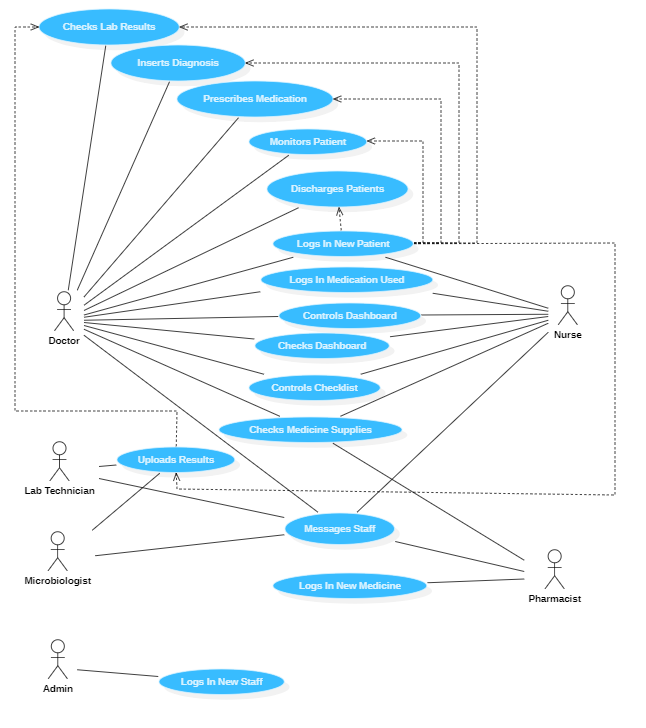
\includegraphics[width=1.0\textwidth]{UML.png}
        \end{figure}
        
        \vspace{0.5cm}

\section{Use Case 1: Διάγνωση Ασθενούς}

Παρακάτω θα αναλυθεί το σενάριο χρήσης του \textbf{Medic World} κατά το οποίο ένας γιατρός καταχωρεί την διάγνωση στην καρτέλα ενός ασθενούς.

\subsection{Περιγραφή}

\begin{center}
     \begin{tabular}{|l|l|}
     \hline
      \textbf{Περίπτωση Χρήσης 1} & Ο γιατρός εισάγει τη διάγνωση ενός ασθενούς \T\B \\ 
      \hline
      \textbf{Ηθοποιός} & Γιατρός \T\B \\
      \hline
      \textbf{Σενάριο Περίπτωσης Χρήσης} & Ένας από τους ασθενείς χρείαζεται διάγνωση, οπότε \T\\& ο γιατρός εισέρχεται στην καρτέλα του, μελετάει τα\\& αποτελέσματα των εξετάσεών και συμπτώματα του και \\& καταλήγει σε διάγνωση \B \\
      \hline
      \textbf{Αφορμή} & Ασθενής χρειάζεται διάγνωση \T\B \\
      \hline
      \textbf{Προαπαιτούμενο 1} & Να έχει καταχωρηθεί ο ασθενής στο σύστημα \T\B \\
      \hline
      \textbf{Προαπαιτούμενο 2} & Να είναι έτοιμα τα αποτελέσματα των εργαστηριακών εξετάσεων \T\B \\
      \hline
     \end{tabular}
 \end{center}
 
 \subsection{Αναλυτικό Σενάριο Χρήσης}
 
 \begin{center}
     \begin{tabular}{|l|l|}
     \hline
      \textbf{Περιγραφή} & Αυτό το σενάριο περιγράφει μια κατάσταση όπου χρειάζεται \T \\& η πλοήγηση σε τέσσερις καρτέλες, οι οποίες τελικά\\& οδηγούν στην επίτευξη του στόχου. \B \\ 
      \hline
      \textbf{Βήμα 1} & Ο γιατρός από το κεντρικό μενού επιλέγει το εικονίδιο \T \\& "Patients" και το σύστημα τον κατευθύνει στην λίστα των ασθενών \B \\
      \hline
      \textbf{Βήμα 2} & Πλοηγείται στην καρτέλα και επιλέγοντας το όνομα του ασθενούς \T \\& κατευθύνεται στο προφίλ του  \B \\
      \hline
      \textbf{Βήμα 3} & Ελέγχει τις ζωτικές ενδείξεις του ασθενούς \T\B \\
      \hline
      \textbf{Βήμα 4} & Επιλέγοντας την ένδειξη "Patient's Profile" κατευθύνεται στο \T\\& ιστορικό του ασθενούς, το οποίο και μελετάει \B \\
      \hline
      \textbf{Βήμα 5} & Επιλέγοντας την ένδειξη "Lab Results" κατευθύνεται \T \\& στα αποτελέσματα εξετάσεων του ασθενούς \B \\
      \hline
      \textbf{Βήμα 6} & Επιλέγει τις εικόνες των εξετάσεων, για να τις μελετήσει \T\B \\
      \hline
      \textbf{Βήμα 7} & Επιλέγοντας την ένδειξη "Diagnosis" εμφανίζεται αναδυόμενο \T \\& παράθυρο με πιθανές ασθένειες \B \\
      \hline
      \textbf{Βήμα 8} & Μελετά την λίστα και επιλέγει την αντίστοιχη ασθένεια\T\B \\
      \hline      
      \textbf{Βήμα 9} & Κατευθύνεται στο παράθυρο ολοκλήρωσης της διάγνωσης \T\B \\
      \hline
      \textbf{Βήμα 10} & Εφαρμόζει τις κατάλληλες τροποποιήσεις \T\B \\
      \hline
      \textbf{Βήμα 11} & Πατάει το κουμπί επιβεβαίωσης \T\B \\
      \hline
      \textbf{Βήμα 12} & Εμφανίζεται αναδυόμενο παράθυρο με την ένδειξη "Επιτυχής Καταχώρηση" \T\B \\
      \hline    
      \textbf{Βήμα 13} & Επιλέγει το κουμπί "ΟΚ"\T\B \\ 
      \hline
      \textbf{Βήμα 14} & Ενημερώνεται το σύστημα και το προφίλ του ασθενούς \T\B \\
      \hline
     \end{tabular}
 \end{center}
 
 \vspace{0.1cm}
 
 \underline{Εναλλακτική Ροή}: \vspace{0.005cm} \\
\par Βήμα 8.1: Δεν τον ικανοποιεί η λίστα των πιθανών ασθενειών, επομένως \parεπιλέγει την έξοδο από το παράθυρο\\
\par Βήμα 9.1: Κατευθύνεται στο παράθυρο ολοκλήρωσης της διάγνωσης\\
\par Βήμα 10.1: Εισάγει τη διάγνωση του \\

 
 \section{Use Case 2: Απασχόληση Χειρουργείου}
 
 Παρακάτω θα αναλυθεί το σενάριο χρήσης του \textbf{Medic World} κατά το οποίο ένας χρήστης επιθυμεί να δηλώσει στο σύστημα τη χρήση ενός χειρουργείου.

\subsection{Περιγραφή}

\begin{center}
     \begin{tabular}{|l|l|}
     \hline
      \textbf{Περίπτωση Χρήσης 2} & Ο χρήστης δηλώνει την απασχόληση χειρουργείου \T\B \\ 
      \hline
      \textbf{Ηθοποιός} & Γιατρός \T\B \\
      \hline
      \textbf{Σενάριο Περίπτωσης Χρήσης} & Ένας γιατρός πρόκειται να εισάγει έναν ασθενή \T \\& σε κάποιο χειρουργείο και χρειάζεται να καταχωρηθεί\\& στην καρτέλα των χειρουργείων ότι το συγκεκριμένο\\& δωμάτιο δε θα είναι διαθέσιμο για κάποιο χρονικό διάστημα \B \\
      \hline
      \textbf{Ηθοποιοί} & Γιατρός, Νοσηλευτής \T\B \\
      \hline
      \textbf{Αφορμή} & Ασθενής χρειάζεται χειρουργείο \T\B \\
      \hline
      \textbf{Προαπαιτούμενο 1} & Να έχει καταχωρηθεί ο ασθενής στο σύστημα \T\B \\
      \hline
      \textbf{Πρoαπαιτούμενο 2} & Να έχει πραγματοποιηθεί διάγνωση του ασθενούς \T\B \\
      \hline
      \textbf{Προαπαιτούμενο 3} & Η διάγνωση να απαιτεί την εισαγωγή σε χειρουργείο \T\B \\
      \hline
     \end{tabular}
 \end{center}
 
 \subsection{Αναλυτικό Σενάριο Χρήσης}
 
 \begin{center}
     \begin{tabular}{|l|l|}
     \hline
      \textbf{Περιγραφή} & Αυτό το σενάριο περιγράφει μια κατάσταση όπου χρείαζεται \T \\& η πλοήγηση σε τρεις καρτέλες, οι οποίες οδηγούν στην \\& επίτευξη του στόχου. \B \\ 
      \hline
      \textbf{Βήμα 1} & Ο χρήστης από το κεντρικό μενού επιλέγει το εικονίδιο  ”Checklist" \T \\& και το σύστημα τον κατευθύνει στην αντίστοιχη οθόνη \B \\
      \hline
      \textbf{Βήμα 2} & Ο χρήστης επιλέγει από το μενού του Checklist \T  τα "Operating Rooms" \T \\& και οδηγείται σε οθόνη που εμφανίζονται όλα τα χειρουργεία διαθέσιμα\\& και μη, με τις αντίστοιχες ενδείξεις \B \\
      \hline
      \textbf{Βήμα 3} & Ο χρήστης ελέγχει τη διαθεσιμότητα των χειρουργείων \T\B \\
      \hline
      \textbf{Βήμα 4} & Ο χρήστης επιλέγει ένα από τα διαθέσιμα χειρουργεία \T\B \\
      \hline
      \textbf{Βήμα 5} & Ο χρήστης οδηγείται σε μία φόρμα συμπλήρωσης στοιχείων \T\B \\
      \hline
      \textbf{Βήμα 6} & Πληκτρολογώντας το όνομα του γιατρού στον χρήστη εμφανίζονται προτάσεις \T \\& από χειρούργους γιατρούς ήδη καταγεγραμμένους στο σύστημα \B \\
      \hline
      \textbf{Βήμα 7} & Πληκτρολογώντας το όνομα του ασθενούς στον χρήστη εμφανίζονται προτάσεις \T \\& από ασθενείς ήδη καταχωρημένους στο σύστημα \B \\
      \hline      
      \textbf{Βήμα 8} & Ο χρήστης πληκτρολογεί την εγχείρηση που πρόκειται να πραγματοποιηθεί \T\B \\   
      \hline
      \textbf{Βήμα 9} & Ο χρήστης μέσω του πλήκτρου "Done" επιλέγει την \T \\& ολοκλήρωση της διαδικασίας \B \\
      \hline
      \textbf{Βήμα 10} & Εμφανίζεται αναδυόμενο παράθυρο με την ένδειξη "Επιτυχής Καταχώρηση" \T\B \\
      \hline
      \textbf{Βήμα 11} & Ενημερώνεται το σύστημα και στην καρτέλα διαθεσιμότητας των χειρουργείων \T \\& εμφανίζεται πλέον ως μη διαθέσιμο το χειρουργείο που επέλεξε νωρίτερα ο χρήστης \B \\
      \hline
     \end{tabular}
 \end{center}
 
\newpage
 
\underline{Εναλλακτική Ροή 1}: \vspace{0.005cm} \\
\par Βήμα 7.1: O ασθενής δεν είναι καταγεγραμμένος στο σύστημα (λόγω επείγοντως περιστατικού), \par επομένως καταχωρείται η επιλογή "not registered"

\vspace{0.3cm}

\underline{Εναλλακτική Ροή 2}: \vspace{0.005cm} \\
\par Βήμα 8.2: Πληκτρολογεί λανθασμένα την εγχείρηση και το σύστημα του εμφανίζει πιθανές διορθώσεις, \par από τις οποίες μπορεί να επιλέξει κάποια 

 

\section{Use Case 3: Καταχώρηση Νέου Φαρμάκου }
 
 Παρακάτω θα αναλυθεί το σενάριο χρήσης του \textbf{Medic World} κατά το οποίο ένας φαρμακοποιός επιθυμεί να εισάγει στο σύστημα ένα νέο φάρμακο.
 
\subsection{Περιγραφή}

\begin{center}
     \begin{tabular}{|l|l|}
     \hline
      \textbf{Περίπτωση Χρήσης 3} & Ο χρήστης εισάγει νέο φάρμακο στην καρτέλα προμηθειών \T\B \\ 
      \hline
      \textbf{Ηθοποιός} & Φαρμακοποιός \T\B \\
      \hline
      \textbf{Σενάριο Περίπτωσης Χρήσης} & Έχει γίνει από το νοσοκομείο αγορά ενός νέου φαρμάκου \T \\& και ο φαρμακοποιός καλείται να το καταχωρήσει \\& στην καρτέλα προμηθειών \B \\
      \hline
      \textbf{Αφορμή} & Η αγορά νέου φαρμάκου \T\B \\
      \hline
      \textbf{Προαπαιτούμενο 1} &  Να μην υπάρχει ήδη το φάρμακο στην καρτέλα προμηθειών \T\B \\
      \hline
     \end{tabular}
 \end{center}
 
 \subsection{Αναλυτικό Σενάριο Χρήσης}
 
 \begin{center}
     \begin{tabular}{|l|l|}
     \hline
      \textbf{Περιγραφή} & Αυτό το σενάριο περιγράφει μια κατάσταση όπου χρειάζεται \T \\& πλοήγηση σε δύο καρτέλες. οι οποίες οδηγούν στην επίτευξη \\& του στόχου \B \\ 
      \hline
      \textbf{Βήμα 1} & Ο φαρμακοποιός από το κεντρικό μενού επιλέγει το εικονίδιο ”Supplies” \T \\& και το σύστημα τον κατευθύνει στην αντίστοιχη οθόνη\\
      \hline
      \textbf{Βήμα 2} & Επιλέγοντας το πλήκτρο "New Medicine" κατευθύνεται στη φόρμα \T \\& συμπλήρωσης του νέου φαρμάκου \B \\
      \hline
      \textbf{Βήμα 3} & Πληκτρολογώντας τη κατηγορία του φαρμάκου στον χρήστη εμφανίζονται προτάσεις \T \\& από τις υπάρχουσες κατηγορίες (λ.χ. αντιβιοτικό), από τις οποίες πρέπει να επιλέξει κάποια \B \\
      \hline
      \textbf{Βήμα 4} & Ο φαρμακοποιός καταχωρεί το όνομα του φαρμάκου \T\B \\
      \hline
      \textbf{Βήμα 5} &  Ο φαρμακοποιός συμπληρώνει τα τεμάχια που προμηθεύτηκαν \T\B \\
      \hline
      \textbf{Βήμα 6} & Στο πλαίσιο "Minimum" συμπληρώνει την ελάχιστη ποσότητα που το σύστημα θα \T \\& αναγνωρίζει ως fully stocked για το συγκεκριμένο φάρμακο \B \\
      \hline
      \textbf{Βήμα 7} & Στο πλαίσιο "Mediocre" συμπληρώνει την ποσότητα που το σύστημα θα \T \\& αναγνωρίζει ως semi stocked για το συγκεκριμένο φάρμακο\\
      \hline
      \textbf{Βήμα 8} & Στο πλαίσιο "Low" συμπληρώνει τη μέγιστη ποσότητα που το σύστημα θα \T \\& αναγνωρίζει ως out of stock για το συγκεκριμένο φάρμακο \B \\
      \hline
      \textbf{Βήμα 9} & Ο φαρμακοποιός επιλέγει το κουμπί "Done" \T\B \\
      \hline
      \textbf{Βήμα 10} & Εμφανίζεται αναδυόμενο παράθυρο με την ένδειξη "Επιτυχής Καταχώρηση" \T\B \\
      \hline    
      \textbf{Βήμα 11} & Γίνεται καταχώρηση στο σύστημα και στην καρτέλα διαθεσιμότητας φαρμάκων, \T \\& επιλέγοντας την κατηγορία  που αφορά το νεοεισαχθέν φάρμακο, εμφανίζεται πλέον το νέο προϊόν \B \\
      \hline
     \end{tabular}
 \end{center}
 
 \newpage
 
  \underline{Εναλλακτική Ροή 1}: \vspace{0.005cm} \\
\par Βήμα 3.1: Η κατηγορία φαρμάκου που πληκτρολόγησε ο χρήστης δεν υπάρχει στο σύστημα, συνεπώς \par αυτομάτως δημιουργείται νέα κατηγορία

\vspace{0.3cm}
 
 \underline{Εναλλακτική Ροή 2}: \vspace{0.005cm} \\
\par Βήμα 4.2: Το φάρμακο που συμπλήρωσε ο χρήστης είναι ήδη καταχωρημένο, με αποτέλεσμα \par το σύστημα αυτομάτως να κλειδώνει και να μη του επιτρέπει τη συνέχεια της διαδικασίας εώς ότου \par διορθωθεί το όνομα



\end{document}
